\documentclass[conference]{IEEEtran}
\IEEEoverridecommandlockouts
\usepackage{cite}
\usepackage{amsmath,amssymb}
\usepackage{graphicx}
\usepackage{booktabs}
\usepackage{multirow}
\usepackage{xcolor}
\usepackage{tikz}
\usetikzlibrary{positioning,arrows.meta,shapes.geometric,fit}
\usepackage{pgfplots}
\pgfplotsset{compat=1.16}
\usepackage[hidelinks]{hyperref}

\newcommand{\mF}{macro-F1}

\begin{document}

\title{Improving Cross-Domain Generalization in Leakage-Safe Bearing Fault Diagnosis:
Reproduction, Negative Results for Domain Adaptation, and Physics-Informed Features That Transfer}

\author{\IEEEauthorblockN{Aryan Saraogi (2023A4PS0427P)}
\IEEEauthorblockA{Birla Institute of Technology and Science (BITS) Pilani\\
ME G545 Course Project\\
Code and results: \url{https://github.com/duetiful/leakage-safe-bearing-fd}}}

\maketitle

\begin{abstract}
Reported accuracies in bearing fault diagnosis are often inflated by data leakage, most
commonly when windows of the same physical bearing appear in both training and test sets.
Domain adaptation (DA) studies in this field usually transfer across operating conditions or
machines while reusing the same bearings. We first define the domain shifts in a recent
leakage-safe benchmark and show that its cross-condition scenarios test on bearings seen in
training, while its Paderborn (PU) Cross-Bearing Instance scenario, where a logistic regression
(LR, \mF{} 0.355) beats the best deep model (0.326), is a true domain-generalization task with
each bearing as a domain. On that task we find, step by step, that (i) the benchmark's models
silently use motor-current channels, and vibration-only input raises both baselines by 0.12;
(ii) a bearing-leaky split lifts the 1D CNN from 0.315 to 0.999; (iii) DANN and SimCLR do not
beat LR, which we explain by the coupling of bearing and label, the lack of target data and
blind model selection; (iv) physics-informed envelope-order features with boosted trees raise
\mF{} from 0.355 to 0.528 across ten rotated bearing hold-outs (9 of 10 folds better, $p=0.004$);
and (v) after a data audit, training on healthy and real-damage bearings with despiked input
reaches 0.590 on the benchmark split and $0.570\pm0.091$ across folds; (vi) a feature-space
analysis shows that the CNN encodes bearing identity three times more than the envelope
features, and that DANN barely reduces it while making classes less compact. Protocols and judging
rules were fixed before results were seen; post-hoc steps are labelled as such.
\end{abstract}

\begin{IEEEkeywords}
bearing fault diagnosis, data leakage, domain generalization, envelope analysis, Paderborn dataset, reproducibility
\end{IEEEkeywords}

\section{Introduction}
Rolling-element bearings are among the most common causes of failure in rotating machinery,
and vibration-based deep learning routinely reports accuracies above 99\% on public datasets.
These numbers rarely survive deployment. A large part of the gap is \emph{data leakage}:
Kapoor and Narayanan documented it in at least 294 papers across 17 fields \cite{kapoor2023},
and Vieira et~al.\ report that earlier reviews found data-splitting problems in over 90\% of
bearing diagnosis papers \cite{vieira2026}. The most common form here is \emph{bearing-level
leakage}: windows of one physical bearing appear in both training and test sets, so the model
is tested on a bearing it has already seen.

Knap et~al.\ \cite{knap2026} built a leakage-safe benchmark (\textit{pdm-bench}) with six
cross-domain scenarios on CWRU and Paderborn (PU). On PU Cross-Bearing Instance their best deep
model reached \mF{} $0.326\pm0.008$ and a logistic regression (LR) 0.355. We take this
scenario as our problem (Sec.~\ref{sec:problem}) and ask:
\textbf{RQ1} Can these baselines be reproduced?
\textbf{RQ2} Does DA let a deep model beat the simple baseline under the same protocol?
\textbf{RQ3} Which single change is responsible for any gain?

Our contributions are: (1) a precise definition of the domain-shift tasks in the benchmark and a
bearing-level leakage audit showing that its cross-condition scenarios reuse training bearings;
(2) a reproduction with a quantified leaky-versus-safe contrast; (3) a pre-registered negative
result for DANN and SimCLR, with an analysis of why; (4) physics-informed envelope-order
features that transfer to unseen bearings on ten rotated hold-outs; and (5) a data audit with a
training-set curation that improves transfer further. Each step's gain or loss is reported in
the order it was made (Fig.~\ref{fig:waterfall}).

\section{Domain Shift in Bearing Diagnosis: Prior Work}\label{sec:prior}
\textbf{Definitions.} Following \cite{chen2023}, a \emph{domain} is a joint distribution
$P(\mathbf{x},y)$ over signal windows $\mathbf{x}$ and fault labels $y$. A model is trained on
source domains and scored on a target domain whose distribution differs. In \emph{unsupervised
domain adaptation} (UDA) unlabeled target windows are available during training; in
\emph{domain generalization} (DG) the target is never seen. The shift can come from the
\emph{operating condition} (speed, load), the \emph{machine} (rig, sensor, bearing type), or the
\emph{bearing instance} (another bearing of the same type with its own defect).

\textbf{How the state of the art does it.} Most published work studies \emph{cross-condition}
UDA on CWRU: train at one motor load, adapt to another, often above 95\% accuracy. WDCNN
re-estimates BatchNorm statistics on the target (AdaBN) \cite{zhang2017wdcnn}; DANN
\cite{ganin2015} adds a domain classifier behind a gradient reversal layer, motivated by the
bound of Ben-David et~al.\ \cite{bendavid2010}, which limits target error by source error plus a
source--target divergence; MMD-based methods \cite{long2015} align feature moments instead.
\emph{Cross-machine} transfer combines both: DCTLN \cite{guo2019} uses a domain classifier and
MMD to move between CWRU, IMS and a railway rig, and Yang et~al.\ \cite{yang2019} transfer from
laboratory bearings to locomotive bearings. When no target data exist, DG methods learn from
several source domains, for example several operating conditions \cite{li2020dg}.
These works inspired our Phase 2: the same DANN and contrastive (SimCLR \cite{chen2020simclr})
machinery, applied to the benchmark's hardest scenario.

\textbf{The gap.} In nearly all of these studies, source and target come from \emph{the same
physical bearings}: each CWRU load condition is recorded on the same seeded-fault bearings. A
model can therefore succeed by recognizing the bearing rather than the fault, which is the
leakage Vieira et~al.\ \cite{vieira2026} warn about; they also find that PU performance rises with
the number of distinct training bearings, not with model capacity. Knap et~al.\ \cite{knap2026}
made splits leakage-safe at the recording level and forbid target data, so every pdm-bench
scenario is a DG task.

\section{Problem Definition}\label{sec:problem}
\noindent\fbox{\parbox{\dimexpr\columnwidth-2\fboxsep-2\fboxrule}{\small
\textbf{Problem taken on.} Can a fault classifier trained on 28 Paderborn bearings diagnose four
bearings it has never seen (pdm-bench PU Cross-Bearing Instance), and can domain adaptation make a
deep model do this better than a logistic regression?\\[2pt]
\textbf{Why this problem.} (1) \emph{It is where the benchmark exposed a gap.} Deep models win
five of the six pdm-bench scenarios, but three of those five reuse training bearings; on this
bearing-safe scenario the best CNN (0.326) loses to LR (0.355). (2) \emph{It is the deployment
case}: the monitored bearing is never in the training data. (3) \emph{It is where DA should
help most}: every bearing is its own domain, yet DA had not been tested across bearings under a
leakage-safe protocol (Sec.~\ref{sec:prior}).}}
\vspace{2pt}

Table~\ref{tab:tasks} lists the benchmark's six tasks with the factor that changes between
source and target. Our bearing-level audit (Sec.~\ref{sec:protocol}) adds the last column: no
recording is shared in any scenario, but CWRU Cross-Load, CWRU Cross-FS and PU Cross-Operating
Condition test entirely on bearings seen in training. They have the highest published
scores (Cross-Load: 1.000) but measure robustness to a new load or sampling rate on a
\emph{known} bearing. No scenario crosses machines.

\begin{table}[t]
\centering
\caption{The six pdm-bench tasks \cite{knap2026} and our bearing-level audit}
\label{tab:tasks}
\setlength{\tabcolsep}{2.5pt}
\resizebox{\columnwidth}{!}{\begin{tabular}{llllc}
\toprule
Scenario & Shift & Source $\rightarrow$ target & Test rec. & Shared bearings \\
\midrule
CWRU Cross-Load & load & 1797/1772/1750 $\rightarrow$ 1730 rpm & 16 & \textbf{16 of 16} \\
CWRU Cross-FS & sampling rate & 12 kHz $\rightarrow$ 48 kHz & 52 & \textbf{13 of 13} \\
CWRU Cross-Fault Inst. & fault size & 0.007/0.014 $\rightarrow$ 0.021 in & 20 & 0 \\
PU Cross-Op.\ Cond. & speed, load & 3 conditions $\rightarrow$ N09\_M07\_F10 & 640 & \textbf{32 of 32} \\
PU Cross-Damage Prov. & damage origin & artificial $\rightarrow$ real damage & 960 & 0 \\
\textbf{PU Cross-Bearing Inst.} & \textbf{bearing} & \textbf{28 bearings $\rightarrow$ 4 new} & 320 & 0 \\
\bottomrule
\multicolumn{5}{l}{\footnotesize No recording is shared in any scenario. All tasks are DG: no target data in training.}
\end{tabular}}
\end{table}

\textbf{Our task.} We study PU Cross-Bearing Instance as domain generalization with each
physical bearing as a domain. Let $\mathcal{B}$ be the 32 PU bearings, $\mathcal{T}=\{$K001,
KA30, KI21, KB23$\}$ the target bearings and $\mathcal{S}=\mathcal{B}\setminus\mathcal{T}$ the 28
source bearings. Bearing $b$ yields windows $\mathbf{x}\in\mathbb{R}^{8192}$ from all four
operating conditions with label $y_b\in\{$H, IR, OR, multiple$\}$. We learn
$f:\mathbf{x}\mapsto y$ from $\{(\mathbf{x},y_b): b\in\mathcal{S}\}$ only, with
$\mathcal{S}\cap\mathcal{T}=\emptyset$, and score \mF{} on $\mathcal{T}$. Because every
bearing is recorded at both 900 and 1500\,rpm and at two loads, the target also spans all
operating conditions: the model must handle a new bearing \emph{and} varying speed and load.

\textbf{Why not cross-condition or cross-machine?} We chose the bearing-instance shift
deliberately. (i) The benchmark's cross-condition tasks reuse every training bearing
(Table~\ref{tab:tasks}), so a gain there cannot be separated from bearing memorization; a
leakage-safe cross-condition task must hold out bearings \emph{and} a condition at once, which
the benchmark does not define and which leaves very few test recordings per class on PU.
(ii) A cross-machine task (e.g.\ CWRU $\rightarrow$ PU) changes bearing type (6205 vs 6203),
sensor position, sampling rate and the label set at once, and pdm-bench has no such scenario
to compare against. Both alternatives are listed as future
work (Sec.~\ref{sec:future}).

\section{Dataset}
\subsection{What a bearing fault looks like}
A rolling-element bearing has an inner ring (fixed to the shaft), an outer ring (fixed to the
housing), and $n$ balls held in a cage. When a defect exists on a surface, each ball striking it
produces a short impact that excites high-frequency structural resonances. The impacts repeat at a
rate set only by the geometry and the shaft frequency $f_r$:
\begin{align}
\mathrm{BPFO} &= \tfrac{n}{2} f_r \left(1-\tfrac{d}{D}\cos\phi\right),\quad
\mathrm{BPFI} = \tfrac{n}{2} f_r \left(1+\tfrac{d}{D}\cos\phi\right),\nonumber\\
\mathrm{BSF} &= \tfrac{D}{2d} f_r \left(1-\left(\tfrac{d}{D}\cos\phi\right)^2\right),
\end{align}
for the outer race, inner race and ball, with ball diameter $d$, pitch diameter $D$ and contact
angle $\phi$. For the type 6203 bearing used in PU ($n=8$, $d=6.75$\,mm, $D=28.55$\,mm,
$\phi=0$), BPFO $=3.054f_r$, BPFI $=4.946f_r$ and BSF $=1.997f_r$. Expressed in multiples of
shaft speed (``orders''), these numbers are the same for every 6203 bearing, which is the
physical reason a model reading them could transfer to a new bearing. In the raw spectrum these low frequencies are buried under shaft, gear and electrical components, and the fault energy sits instead at the kHz resonances that the impacts excite. Envelope analysis band-passes the signal around a resonance and demodulates it, which recovers the impact \emph{rate} \cite{randall2011}. An inner-ring defect also
rotates with the shaft, so its impacts are modulated at $f_r$, creating sidebands at
BPFI\,$\pm f_r$.




\subsection{The Paderborn (PU) dataset}



The PU dataset \cite{lessmeier2016} was recorded on a rig with a drive motor, torque shaft,
bearing test module and load motor. Its 32 type-6203 bearings are 6 healthy (K001--K006), 12 with \emph{artificial} damage
from electric discharge machining, drilling or engraving (7 outer ring, 5 inner ring), and 14
with \emph{real} damage from accelerated lifetime tests (5 outer, 6 inner, 3 multiple). They are each recorded under
four operating conditions combining speed (900 or 1500\,rpm), load torque (0.1 or 0.7\,Nm) and
radial force (400 or 1000\,N), 20 recordings of 4\,s each, with housing vibration at 64\,kHz
alongside two motor phase currents. Classes come from the bearing code: healthy (K), outer ring
(KA), inner ring (KI) and multiple (KB). Recordings are cut into windows of 8,192 samples
(0.128\,s), with 75\% overlap for training and 50\% for testing \cite{knap2026}. In Cross-Bearing
Instance each test class is a single unseen real-damage bearing, so one bearing flipping changes
\mF{} by up to 0.25, while 12 training bearings carry artificial damage.

\section{Leakage-Safe Protocol}\label{sec:protocol}
\textbf{Split checks.} Our package resolves every scenario from the file lists, exports the
recording lists, and fails if any recording is on both sides; a second check reports shared
\emph{physical} bearings (last column of Table~\ref{tab:tasks}).

\textbf{Metric.} \mF{} is the unweighted mean of per-class F1,
$\mathrm{F1}_c = 2P_cR_c/(P_c+R_c)$, so the healthy class cannot dominate the score.

\textbf{Rotated folds.} Because the benchmark split rests on four bearings, we add nine more
folds, each holding out one random real-damage bearing per fault class plus one healthy bearing
(fixed seed), giving ten folds with fold 0 equal to the benchmark split. Paired comparisons use
a two-sided Wilcoxon signed-rank test over folds.

\textbf{Pre-registration.} Before each phase, its protocol, hyperparameter grid, selection rule
and judging rule were committed to the repository. A method ``works'' only if it beats the
baseline on fold 0 by more than the seed spread ($\approx$0.03) \emph{and} beats it across folds
with $p<0.05$. All hyperparameters are chosen on source bearings only.

\section{Methods and Architectures}
\begin{figure*}[t]
\centering
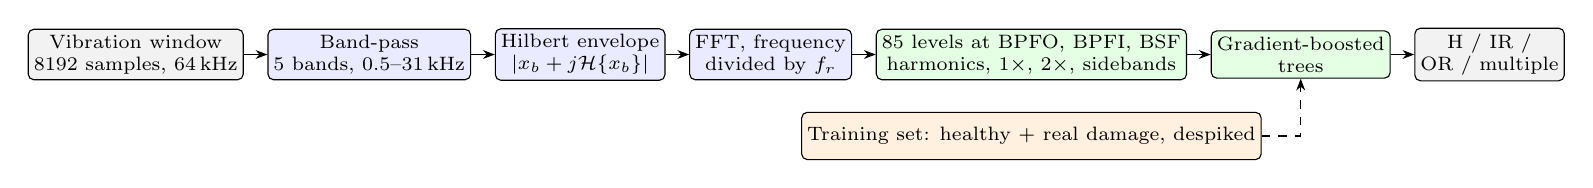
\begin{tikzpicture}[font=\scriptsize, node distance=3mm and 3mm,
  box/.style={draw, rounded corners=2pt, align=center, minimum height=6mm, inner sep=2pt, fill=#1},
  box/.default=white, >={Stealth[length=1.5mm]}]
\node[box=gray!10] (raw) {Vibration window\\8192 samples, 64\,kHz};
\node[box=blue!8, right=of raw] (bp) {Band-pass\\5 bands, 0.5--31\,kHz};
\node[box=blue!8, right=of bp] (env) {Hilbert envelope\\$|x_b + j\mathcal{H}\{x_b\}|$};
\node[box=blue!8, right=of env] (fft) {FFT, frequency\\divided by $f_r$};
\node[box=green!10, right=of fft] (feat) {85 levels at BPFO, BPFI, BSF\\harmonics, $1\times$, $2\times$, sidebands};
\node[box=green!10, right=of feat] (gbt) {Gradient-boosted\\trees};
\node[box=gray!10, right=of gbt] (out) {H / IR /\\OR / multiple};
\node[box=orange!12, below=4mm of feat] (cur) {Training set: healthy + real damage, despiked};
\draw[->] (raw) -- (bp); \draw[->] (bp) -- (env); \draw[->] (env) -- (fft);
\draw[->] (fft) -- (feat); \draw[->] (feat) -- (gbt); \draw[->] (gbt) -- (out);
\draw[->, dashed] (cur.east) -| (gbt.south);
\end{tikzpicture}
\caption{Proposed pipeline. The envelope-order features are read at physically fixed positions,
so they mean the same thing on every 6203 bearing.}
\label{fig:pipe}
\end{figure*}


\subsection{Baselines}
\textbf{Logistic regression (LR)} on hand-crafted time- and frequency-domain statistics (RMS,
kurtosis, crest, shape, clearance and impulse factors, mean frequency, frequency centre, etc.),
standardized, with Bayesian hyperparameter search, as in pdm-bench.

\textbf{1D CNN} (pdm-bench): three convolution blocks, Conv1d(32, $k$=7) $\rightarrow$
Conv1d(64, $k$=5) $\rightarrow$ Conv1d(128, $k$=3), each followed by BatchNorm and ReLU, then
global average pooling and a classifier Linear(128,64)--ReLU--Dropout(0.4)--Linear(64,4).
AdamW (lr $10^{-3}$), batch 64, 50 epochs, last epoch scored, seeds 41--43.

\subsection{Domain adaptation on the same backbone}
\textbf{DANN, bearing adversary (domain generalization).} A domain head
Linear(128,64)--ReLU--Linear(64,$B$) is attached to the 128-d CNN embedding through a gradient
reversal layer $R_\lambda$ (identity forward, $-\lambda\nabla$ backward) \cite{ganin2015}:
\begin{equation}
\min_{\theta_f,\theta_y}\max_{\theta_d}\;
\mathcal{L}_y(\theta_f,\theta_y)-\lambda\,\mathcal{L}_d(\theta_f,\theta_d).
\end{equation}
Since the benchmark forbids target data in training, the domains are the 28 \emph{source}
bearings. In the \emph{within-class} variant the adversary only separates bearings of the
window's own class, so removing bearing identity does not fight the fault label.

\textbf{SimCLR.} The feature extractor is pre-trained with the NT-Xent loss ($\tau=0.2$) on two
augmented views of each source window (random gain, polarity flip, circular shift, noise, time
mask) through a 128--128--64 projection head, then fine-tuned with labels.

Hyperparameters ($\lambda\in\{0.1,1\}$) were chosen on four held-out \emph{source} bearings
(K006, KA22, KB27, KI18) by a fixed rule; the test bearings were never loaded in that stage.

\subsection{Proposed: envelope-order features with boosted trees}
For each window $x(t)$ and each of five bands (0.5--4, 4--10, 10--20, 20--31 and 0.5--31\,kHz),
the band-passed signal $x_b$ is demodulated with the Hilbert transform,
$e_b(t)=|x_b(t)+j\mathcal{H}\{x_b\}(t)|$, and the spectrum of $e_b$ is resampled onto an order
axis $o=f/f_r$ (0.2 to 16, step 0.04), with $f_r$ from the file's nominal speed. Per band we read
the log level, relative to the band's median, at harmonics 1--3 of BSF, BPFO and BPFI, at shaft
orders 1 and 2, and at the BPFI\,$\pm1$ sidebands, plus band energy share and envelope kurtosis:
85 features (Fig.~\ref{fig:pipe}). Because these positions are fixed by physics, not learned
from the training bearings, they should mean the same thing on an unseen bearing. The classifier
is a histogram gradient-boosted tree ensemble (200 iterations, learning rate 0.1, 31 leaves, L2
1.0, balanced class weights), with settings fixed in advance, not tuned.

\subsection{Data curation from an audit (post hoc)}
After Phase 3 we audited per-bearing signal statistics (Sec.~\ref{sec:audit}) and tested two
fixes: \emph{despiking}, which clips each window at 4 robust standard deviations, and
\emph{real-damage-only training}, which drops the 12 artificially damaged bearings so that the
16 remaining training bearings (healthy and real damage) match the test bearings' damage origin.

\textbf{Envelope CNN with AdaBN.} A small CNN (Conv1d 32/64/64) reads the full $5\times395$ log
envelope-order spectrum; AdaBN \cite{li2016adabn} optionally re-estimates its BatchNorm statistics
on each unseen bearing (test-time adaptation, not DG).


\textbf{Implementation.} pdm-bench is a pinned dependency (commit \texttt{ca52408}), so
baselines run on the authors' loaders; all PU and CWRU files are checked against SHA-256
checksums.

\section{Results}
Fig.~\ref{fig:waterfall} shows every step in the order it was made, on the benchmark split,
and Table~\ref{tab:steps} gives the same chain over ten folds. The subsections explain each step.

\begin{figure*}[t]
\centering
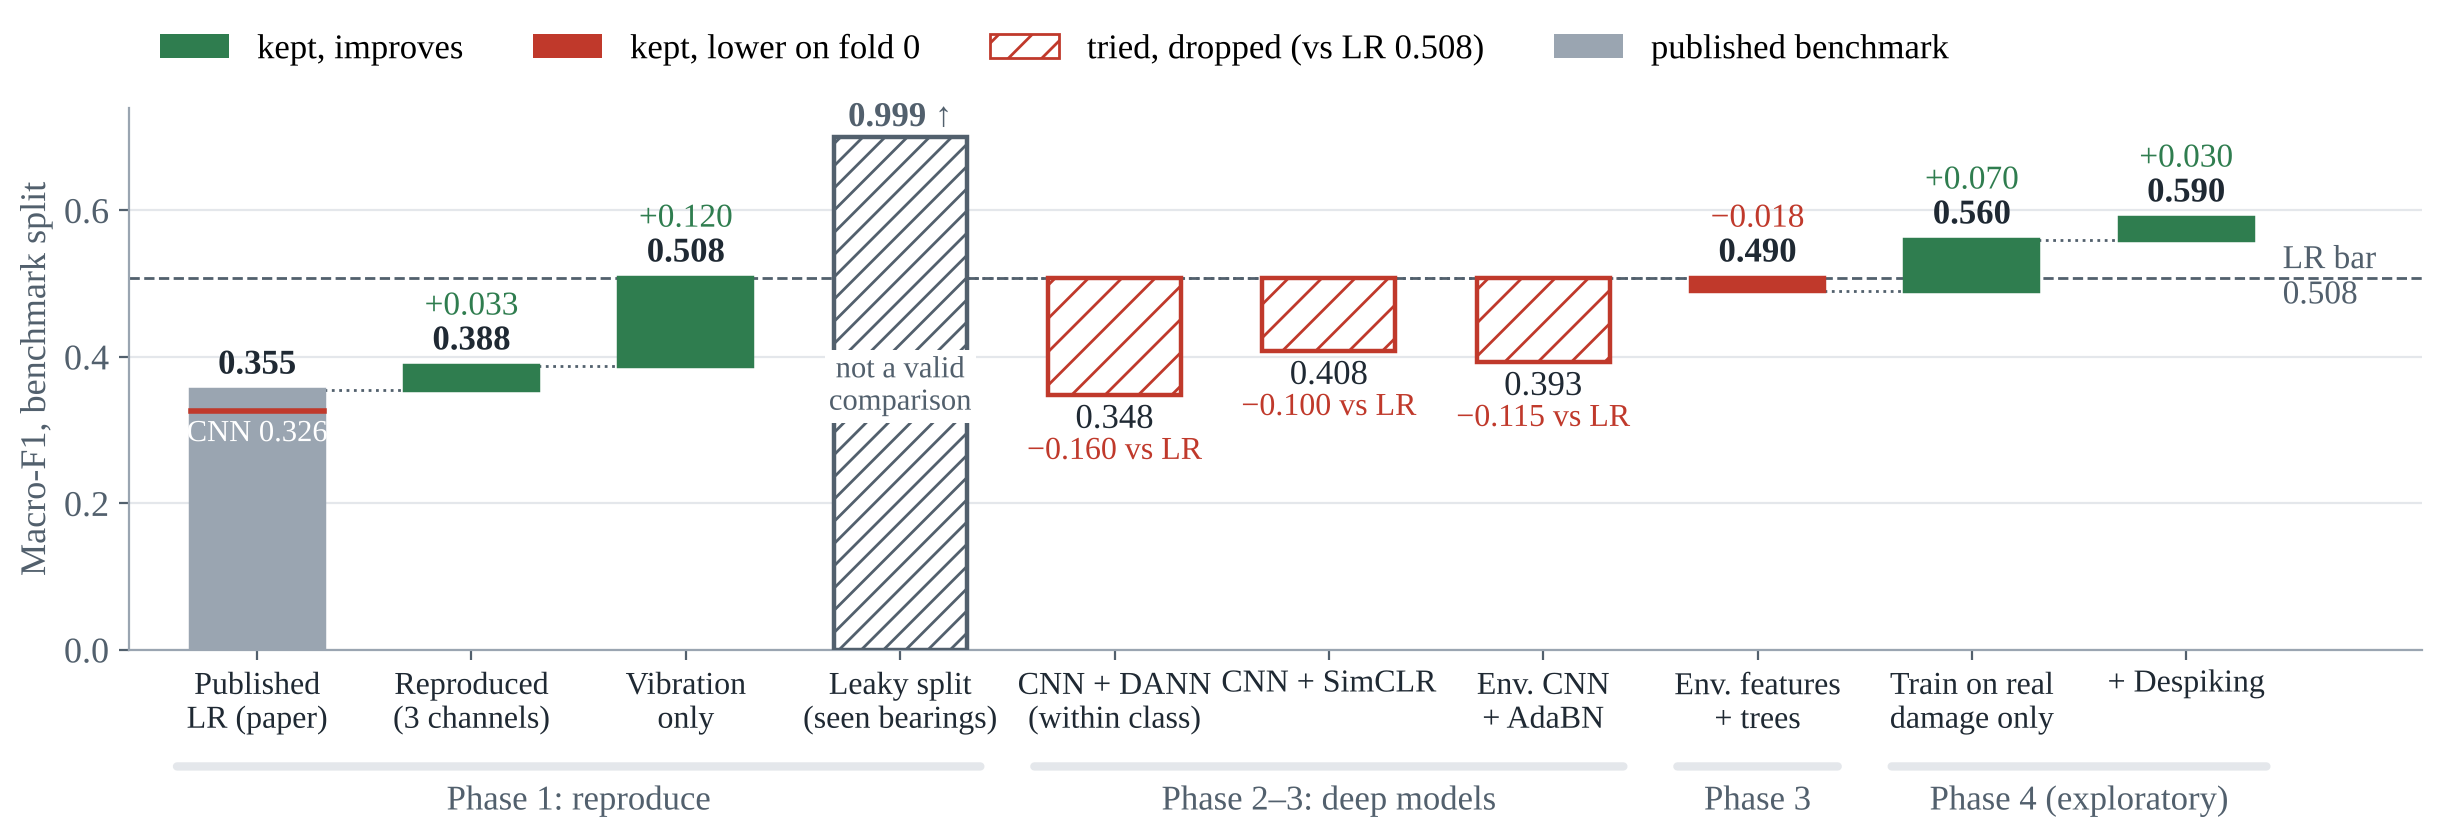
\includegraphics[width=\textwidth]{figs/waterfall_fold0.png}
\caption{Chronological flow of the project on the benchmark split (test bearings K001, KA30,
KI21, KB23). Each bar starts where the previous kept step ended and shows its gain (green) or
loss (red). Hatched red: methods tried against the vibration-only LR bar (0.508) and dropped.
The leaky split is shown for contrast only: it tests on seen bearings and is not a valid result.}
\label{fig:waterfall}
\end{figure*}

\begin{table}[t]
\centering
\caption{Chronological steps over ten rotated bearing hold-outs (\mF{}, mean $\pm$ std over folds; fold 0 is the benchmark split)}
\label{tab:steps}
\setlength{\tabcolsep}{2.5pt}
\resizebox{\columnwidth}{!}{\begin{tabular}{llcccc}
\toprule
Ph. & Change (one at a time) & 10 folds & $\Delta$ & Fold 0 & Better, $p$ \\
\midrule
3 & LR on generic statistics (reference) & $0.355\pm0.101$ & -- & 0.376 & -- \\
3 & \quad classifier $\rightarrow$ trees (generic) & $0.381\pm0.093$ & $+0.026$ & 0.336 & 5/10, 0.63 \\
3 & input $\rightarrow$ envelope-order features (LR) & $0.448\pm0.098$ & $+0.093$ & 0.360 & 8/10, 0.027 \\
3 & classifier LR $\rightarrow$ boosted trees & $0.528\pm0.100$ & $+0.080$ & 0.490 & 9/10, 0.004 \\
4$^\ast$ & train on healthy + real damage only & $0.563\pm0.093$ & $+0.035$ & 0.560 & 9/10, 0.010$^\dagger$ \\
4$^\ast$ & despike input (clip at 4 robust s.d.) & $\mathbf{0.570\pm0.091}$ & $+0.007$ & \textbf{0.590} & 7/10, 0.027$^\dagger$ \\
\midrule
3 & envelope CNN (DG, 3 seeds) & -- & & 0.318 & \\
3 & \quad + AdaBN per test bearing (TTA) & -- & & 0.393 & \\
\bottomrule
\multicolumn{6}{l}{\footnotesize Better/$p$: vs.\ LR generic (Wilcoxon). $^\ast$post hoc. $^\dagger$vs.\ trees/envelope on all bearings.}
\end{tabular}}
\end{table}

\subsection{Reproduction and the cost of leakage (RQ1)}\label{sec:repro}
On the benchmark split (Fig.~\ref{fig:waterfall}, Phase 1) the CNN reproduces within its seed
spread ($0.315\pm0.032$ vs $0.326\pm0.008$); LR scores 0.388 against 0.355 with identical code
and seed, and still beats every CNN seed. Our CNN seed spread is four times the paper's, so any
gain below $\approx$0.03 is noise.

Two audit findings change the picture. First, the released PU loader keeps every channel of the
64\,kHz raster, so all models see two motor currents plus vibration, which the paper does not
state. Using vibration only raises \emph{both} baselines by 0.12 (LR 0.508, CNN
$0.436\pm0.023$); the currents appear to carry rig- or bearing-specific cues that do not
transfer. Second, with a bearing-leaky split (every bearing in training, test on unseen
recordings of them), LR reaches 0.841 and the CNN 0.999 (seed 41). Leakage turns the CNN from
the loser into a near-perfect winner, so a leaky protocol would have reversed the benchmark's
conclusion. The bar for the rest of the project is vibration-only LR, 0.508.

\subsection{Domain adaptation does not help (RQ2)}\label{sec:da}
On the four source validation bearings, the within-class DANN at $\lambda=1$ led ERM by 0.23
(0.527 vs 0.294) and was selected. On the test bearings (3 seeds, 20 epochs to fit free GPU
time, so ERM from the same trainer is the control), ERM scores $0.404\pm0.027$, SimCLR
$0.408\pm0.034$ ($+0.004$) and DANN $0.348\pm0.013$ ($-0.056$), all far below the LR bar of
0.508 (Fig.~\ref{fig:waterfall}). SimCLR is indistinguishable from ERM, DANN is worse by twice
the seed spread, and the setting that won source-only validation by 0.23 was the \emph{worst} on
test. The answer to RQ2 is negative.

\subsection{Why does LR beat DANN?}\label{sec:why}
DA theory predicts that DANN should help, so this result needs explaining. Four properties of
the task break the assumptions behind it.
(1) \emph{The domain is tangled with the label.} Each bearing carries one fault class, so a plain
bearing adversary that makes features bearing-invariant also makes them class-invariant. Zhao
et~al.\ \cite{zhao2019} prove that enforcing invariant features can \emph{increase} target error
when label distributions differ across domains. Our within-class adversary avoids this, but
then it has only 2 to 11 training bearings per class to learn the invariance from (2 for
multiple damage), and it lowered \mF{} from 0.404 to 0.348.
(2) \emph{DG offers no target to align to.} The Ben-David bound \cite{bendavid2010} measures the
divergence to the \emph{target}; in DG, aligning 28 source bearings only helps if an unseen
bearing lies inside their span. Classic source-versus-target DANN (UDA, which the benchmark
forbids) did not help either on our validation bearings (0.309 and 0.200 vs ERM 0.294).
(3) \emph{Capacity enables shortcuts.} The same CNN scores 0.999 when test bearings are seen in
training, so it can memorize bearing-specific cues (resonances, the spike artifact of
Sec.~\ref{sec:audit}); its embedding carries three times the bearing identity of the envelope
features (Sec.~\ref{sec:fs}). LR on 11 summary statistics has little room to memorize a bearing.
(4) \emph{Model selection is blind.} The DANN setting that led source validation by 0.23 was the
worst on test. This pattern is not unique to us: in DomainBed \cite{gulrajani2021}, carefully
tuned ERM matched or beat DANN and most DG methods, and pdm-bench itself found LR above the CNN on
this scenario \cite{knap2026}.
The lesson is that the invariance DANN tries to \emph{learn} from 28 bearings is already known
from physics: fault orders are the same on every 6203 bearing. Phase 3 puts that invariance into
the input instead.

\textbf{Problems faced.} Beyond the negative result, the deep pipeline met practical obstacles:
undocumented motor-current channels in the loader (Sec.~\ref{sec:repro}); a 20-epoch budget on
free GPUs (about 50\,min per run); a plain bearing adversary that fought the label, which led
to the within-class design; and the absence of any target data for UDA under the benchmark's
rules.

\subsection{Physics-informed features transfer (RQ3)}
Table~\ref{tab:steps} reports all ten folds. Changing only the input from generic to
envelope-order features raises LR by $+0.093$ ($p=0.027$) and boosted trees by $+0.147$
($p=0.010$), so the features, not the classifier, carry the gain. The combination reaches
$0.528\pm0.100$, better than the generic-feature LR on 9 of 10 folds ($p=0.004$). Tuning the
trees by leave-bearings-out cross-validation inside the training bearings changes nothing
($0.524$), so the result does not rest on lucky settings.



The gain appears where the physics predicts: averaged over the ten folds, outer-ring F1 rises from
0.12 to 0.56 and inner-ring F1 from 0.24 to 0.56 (LR/generic to trees/envelope); these classes each have one characteristic
frequency. The multiple-damage class, a mixture of both signatures, does not improve.



On fold 0 alone, the trees score 0.490, just below the 0.508 bar, so the strict pre-registered
criterion is \emph{not} met in Phase 3. Fold 0 is fragile (LR on the same features moves
between 0.36 and 0.47 with its regularization), so the 10-fold result is the main evidence.
The envelope CNN overfits the training bearings (0.318); AdaBN lifts it to 0.393, still below
the feature models.

\subsection{Data audit and curated training (exploratory)}\label{sec:audit}
Counting impulses above 8 robust standard deviations revealed a train of spikes at 100\,Hz at
1500\,rpm and 52.5\,Hz at 900\,rpm. The ratio (1.90) is not the speed ratio (1.67) and the
frequency matches no bearing order, so the spikes are not bearing impacts. They are strong in
healthy K001--K003 and K006 (74--225 events/s, up to 77\% of signal energy), weaker in artificial
damage (7--69/s), and nearly absent in real damage (0--5/s). A model can therefore learn
``periodic spikes $\Rightarrow$ healthy or artificial'' instead of fault physics. The healthy bearings
without the artifact are the hardest to recognize (K005 is correct in only 18--23\% of windows).
Despiking lifts trees on \emph{generic} features by $+0.084$ (9 of 10 folds), direct evidence
that generic statistics partly fit the artifact, while envelope features, which read periodicity
at fault orders, are already insensitive to it ($-0.004$).

Training only on healthy and real-damage bearings is the most useful single change: $+0.035$ over
10 folds ($p=0.010$) and 0.560 on fold 0, mostly by recognizing KA30 (plastic indentations, unlike
the drilled or EDM training damage) in 52\% of windows instead of 21\%. With despiking added, the
final model reaches \textbf{0.590 on the benchmark split}, 0.08 above the 0.508 baseline and 0.15
above the 1D CNN, and $0.570\pm0.091$ across folds (Fig.~\ref{fig:waterfall}). Because these choices came from looking at
the data after Phase 3, we report them as exploratory, not as a pre-registered result.

The audit also showed that the dataset authors \cite{lessmeier2016} label KB23 and KB24 as
inner-ring dominant and KB27 as outer-ring dominant, and use three classes. Under those labels
the same model reaches $0.756\pm0.129$ (generic LR 0.501); the 4-class ``multiple'' class is
close to unlearnable across bearings.




\subsection{Feature-space analysis}\label{sec:fs}
A good cross-bearing representation should make the four classes compact and separated while
\emph{not} separating individual bearings of the same class. We designed three measures, all
computed in the full-dimensional space on the same 10{,}236 windows (4 per recording, all 32
bearings), standardized with training-bearing statistics only: the \emph{class silhouette}
(higher is better), the \emph{within-class bearing silhouette} (lower is better: bearing identity
left in the features), and the \emph{kNN-transfer \mF{}}, a 15-nearest-neighbour vote from
training windows to held-out-bearing windows. They are applied to the generic statistics, the
envelope-order features (raw and despiked, all and real-damage bearings), and the 128-d
embeddings of the ERM CNN and the within-class DANN. 2-D maps are UMAP projections fitted
without labels (Fig.~\ref{fig:fs}); every number in Table~\ref{tab:fs} is computed before
projection.

\begin{table}[t]
\centering
\caption{Feature-space compactness and transfer (10{,}236 windows, all 32 bearings)}
\label{tab:fs}
\setlength{\tabcolsep}{2.5pt}
\resizebox{\columnwidth}{!}{\begin{tabular}{lcccc}
\toprule
& \multicolumn{2}{c}{Silhouette} & \multicolumn{2}{c}{kNN-transfer \mF{}} \\
Representation (dim.) & class $\uparrow$ & bearing $\downarrow$ & fold 0 & 10 folds \\
\midrule
Generic statistics (11) & $-0.002$ & 0.070 & 0.352 & $0.432\pm0.095$ \\
\quad despiked & $0.000$ & 0.117 & 0.352 & $\mathbf{0.486\pm0.101}$ \\
Envelope-order (85) & $0.015$ & 0.050 & 0.438 & $0.449\pm0.065$ \\
\quad despiked & $0.022$ & \textbf{0.047} & 0.430 & $0.448\pm0.065$ \\
\quad despiked, real-damage only & $0.031$ & 0.063 & \textbf{0.440} & $0.433\pm0.057$ \\
CNN embedding, ERM (128)$^\ast$ & $\mathbf{0.037}$ & 0.147 & 0.383 & -- \\
DANN embedding (128)$^\ast$ & $0.026$ & 0.134 & 0.313 & -- \\
\bottomrule
\multicolumn{5}{l}{\footnotesize $^\ast$Reduced CPU retrain, one seed; own fold-0 \mF{}: ERM 0.464, DANN 0.410.}
\end{tabular}}
\end{table}

\begin{figure}[t]
\centering
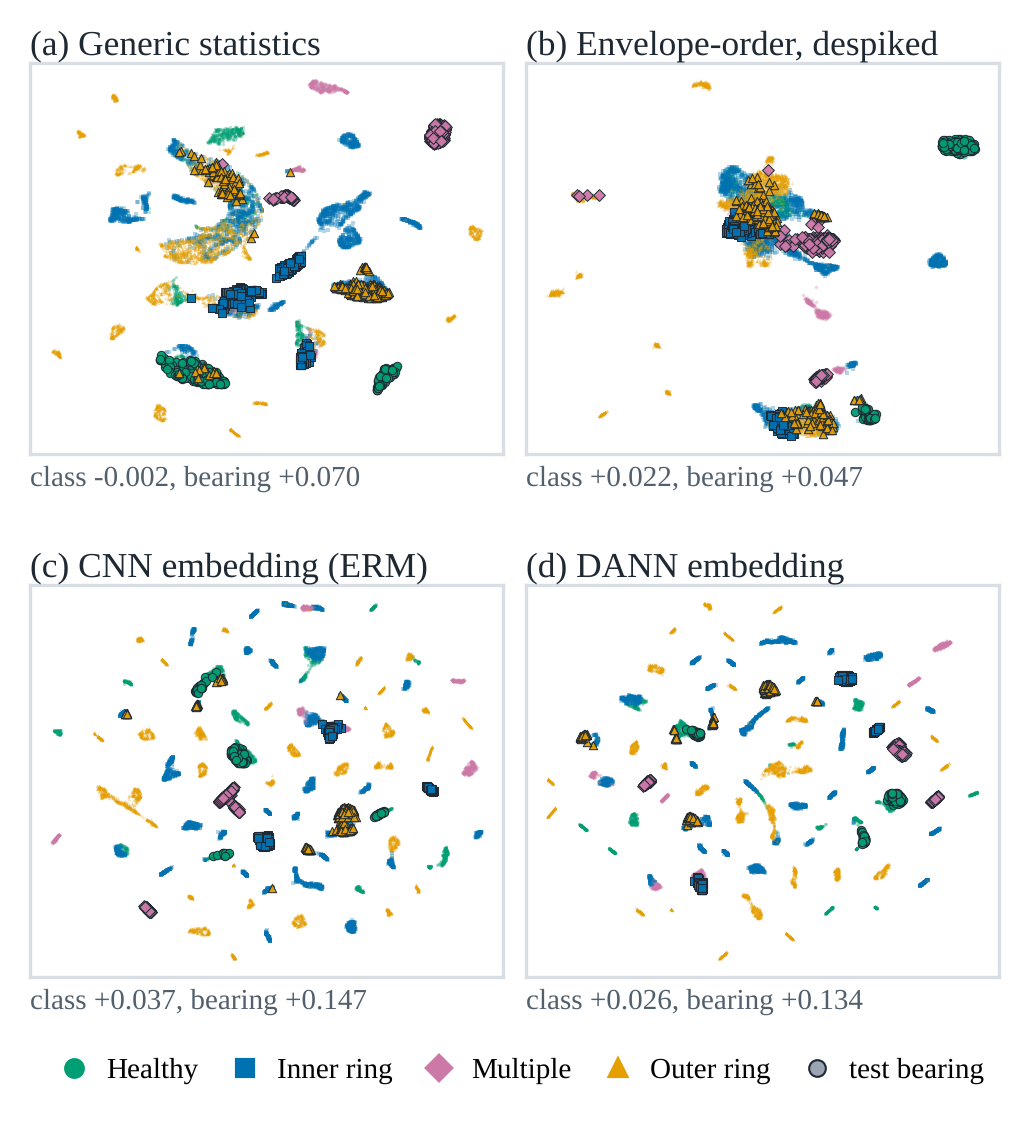
\includegraphics[width=\columnwidth]{figs/fs_maps.png}
\caption{UMAP maps of the same windows in four representations. Small points: training
bearings; outlined: the four unseen test bearings. Under each map: class and within-class
bearing silhouettes. The CNN and DANN spaces break into one island per bearing.}
\label{fig:fs}
\end{figure}

Three findings stand out. (1) \emph{No representation forms compact classes}: every class
silhouette lies between $-0.002$ and 0.037, so the four classes overlap heavily in all spaces,
which is consistent with the modest \mF{} of every model. (2) \emph{The CNN encodes bearing
identity.} Its within-class bearing silhouette (0.147) is three times that of the envelope
features (0.047), and its map splits into one island per bearing (Fig.~\ref{fig:fs}c): the
feature-space picture of the memorization behind the 0.999 leaky score. DANN lowers this only
slightly (0.134) while also lowering class compactness (0.037 $\rightarrow$ 0.026) and kNN
transfer (0.383 $\rightarrow$ 0.313); its own \mF{} falls from 0.464 to 0.410, the same direction
as the three-seed result of Sec.~\ref{sec:da}. (3) \emph{Each feature-side step helps a
little.} Envelope features carry the least bearing identity and place unseen bearings among
training windows of their own class more often on fold 0 (0.43--0.44 vs 0.35); despiking and
real-damage training raise class compactness step by step (0.015 $\rightarrow$ 0.022
$\rightarrow$ 0.031). One result does not fit a simple story: over ten folds, kNN on despiked
\emph{generic} statistics transfers best (0.486), so the trees' gain in Table~\ref{tab:steps}
comes from selecting a few fault-order dimensions, not from the whole space becoming more
compact. The CNN and DANN embeddings come from a reduced CPU retrain (8 epochs, a quarter of
the training windows), as the Phase 2 checkpoints were not kept.

\section{Limitations}
All results are on one dataset (PU) and one scenario; CWRU was used only for the leakage audit.
Feature models are deterministic, so the fold spread ($\approx$0.10) is the uncertainty, and the
rotated folds share bearings (only three KB bearings exist), so $p$-values are indicative. Phase 2
used 20 rather than 50 epochs and three seeds. The final curation step is post hoc. The 0.128\,s window limits envelope resolution to
0.3--0.5 orders. The CNN/DANN embeddings of Sec.~\ref{sec:fs} come from a single reduced retrain.

\section{Future Prospects}\label{sec:future}
(1) \emph{Leakage-safe cross-condition and cross-machine tasks}: hold out bearings \emph{and} an
operating condition together, and transfer across machines (CWRU, Ottawa) by rescaling fault
orders with each bearing's geometry. (2) \emph{Longer windows or recording-level decisions} to
sharpen fault-order resolution. (3) \emph{Physics-guided deep models} constrained to fault-order
positions or trained on the curated set. (4) \emph{Model selection} for unseen bearings by
leave-one-bearing-out validation. (5) \emph{Multi-label targets} \cite{vieira2026} instead of a
``multiple'' class. (6) \emph{More bearings}: bearing diversity, not model size, is the
strongest lever.

\section{Conclusion}
Under a leakage-safe protocol with whole bearings held out, neither a standard 1D CNN nor
domain-adaptation variants beat a logistic regression on PU, and leaky splits would have hidden
this. Physics-informed envelope-order features with boosted trees transfer to unseen bearings
(0.355 $\rightarrow$ 0.528 across ten folds), and curating the training set after a data audit
raises the benchmark score to 0.590. The improvement came from understanding the signal and the
data, not from a larger network.

\begin{thebibliography}{99}
\bibitem{kapoor2023} S. Kapoor and A. Narayanan, ``Leakage and the reproducibility crisis in
machine-learning-based science,'' \emph{Patterns}, vol.~4, no.~9, p.~100804, 2023.
\bibitem{vieira2026} Vieira, Bauler, Rosa and Silva, ``Towards a more realistic evaluation of
machine learning models for bearing fault diagnosis,'' \emph{Mech. Syst. Signal Process.}, 2026,
doi:10.1016/j.ymssp.2026.114640.
\bibitem{knap2026} Knap, Jachymczyk and Lalik, ``Leakage-safe, reproducible benchmarking for
vibration-based fault diagnosis,'' in \emph{Proc. PHM Society European Conf.}, 2026.
\bibitem{chen2023} X. Chen, R. Yang, Y. Xue, M. Huang, R. Ferrero and Z. Wang, ``Deep transfer
learning for bearing fault diagnosis: A systematic review since 2016,'' \emph{IEEE Trans.
Instrum. Meas.}, vol.~72, p.~3508221, 2023.
\bibitem{zhang2017wdcnn} W. Zhang, G. Peng, C. Li, Y. Chen and Z. Zhang, ``A new deep learning
model for fault diagnosis with good anti-noise and domain adaptation ability on raw vibration
signals,'' \emph{Sensors}, vol.~17, no.~2, p.~425, 2017.
\bibitem{ganin2015} Y. Ganin and V. Lempitsky, ``Unsupervised domain adaptation by
backpropagation,'' in \emph{Proc. ICML}, PMLR 37, 2015, pp.~1180--1189.
\bibitem{bendavid2010} S. Ben-David, J. Blitzer, K. Crammer, A. Kulesza, F. Pereira and J. W.
Vaughan, ``A theory of learning from different domains,'' \emph{Mach. Learn.}, vol.~79,
pp.~151--175, 2010.
\bibitem{long2015} M. Long, Y. Cao, J. Wang and M. I. Jordan, ``Learning transferable features
with deep adaptation networks,'' in \emph{Proc. ICML}, 2015, pp.~97--105.
\bibitem{guo2019} L. Guo, Y. Lei, S. Xing, T. Yan and N. Li, ``Deep convolutional transfer
learning network: A new method for intelligent fault diagnosis of machines with unlabeled
data,'' \emph{IEEE Trans. Ind. Electron.}, vol.~66, no.~9, pp.~7316--7325, 2019.
\bibitem{yang2019} B. Yang, Y. Lei, F. Jia and S. Xing, ``An intelligent fault diagnosis
approach based on transfer learning from laboratory bearings to locomotive bearings,''
\emph{Mech. Syst. Signal Process.}, vol.~122, pp.~692--706, 2019.
\bibitem{li2020dg} X. Li, W. Zhang, Q. Ding and J.-Q. Sun, ``Domain generalization in rotating
machinery fault diagnostics using deep neural networks,'' \emph{Neurocomputing}, vol.~403,
pp.~409--420, 2020.
\bibitem{chen2020simclr} T. Chen, S. Kornblith, M. Norouzi and G. Hinton, ``A simple framework
for contrastive learning of visual representations,'' in \emph{Proc. ICML}, 2020.
\bibitem{randall2011} R. B. Randall and J. Antoni, ``Rolling element bearing diagnostics---A
tutorial,'' \emph{Mech. Syst. Signal Process.}, vol.~25, no.~2, pp.~485--520, 2011.
\bibitem{lessmeier2016} C. Lessmeier, J. K. Kimotho, D. Zimmer and W. Sextro, ``Condition
monitoring of bearing damage in electromechanical drive systems by using motor current signals
of electric motors: A benchmark data set for data-driven classification,'' in \emph{Proc. PHM
Society European Conf.}, 2016.
\bibitem{li2016adabn} Y. Li, N. Wang, J. Shi, J. Liu and X. Hou, ``Revisiting batch
normalization for practical domain adaptation,'' arXiv:1603.04779, 2016.
\bibitem{zhao2019} H. Zhao, R. Tachet des Combes, K. Zhang and G. Gordon, ``On learning
invariant representations for domain adaptation,'' in \emph{Proc. ICML}, 2019, pp.~7523--7532.
\bibitem{gulrajani2021} I. Gulrajani and D. Lopez-Paz, ``In search of lost domain
generalization,'' in \emph{Proc. ICLR}, 2021.
\end{thebibliography}

\end{document}
